\chapter{Calibration Model}


\section{Dot Detection Algorithm}

A common method used to calibrate a stereo vision system is to use a calibration plate. The computer vision system then needs to determine where the dots on the plate are. This can be achieved in many ways, but one of the most reliable methods is the ‘Gaussian Peak’ detection method. In this approach, a 2D Gaussian object is used as a template and passed over a search region to identify peaks, in our case ‘dots’ or bright spots. Figure \ref{fig:gaussian_dis} shows the two dimensions gaussian template. We compute the cross correlation of the template with our calibration plate and finally detect the dots with `+' mark as shown in Figure \ref{fig:dot_detect}.

\begin{figure}[h!]
	\centering
	\begin{subfigure}[t]{0.45\linewidth}
		\centering
		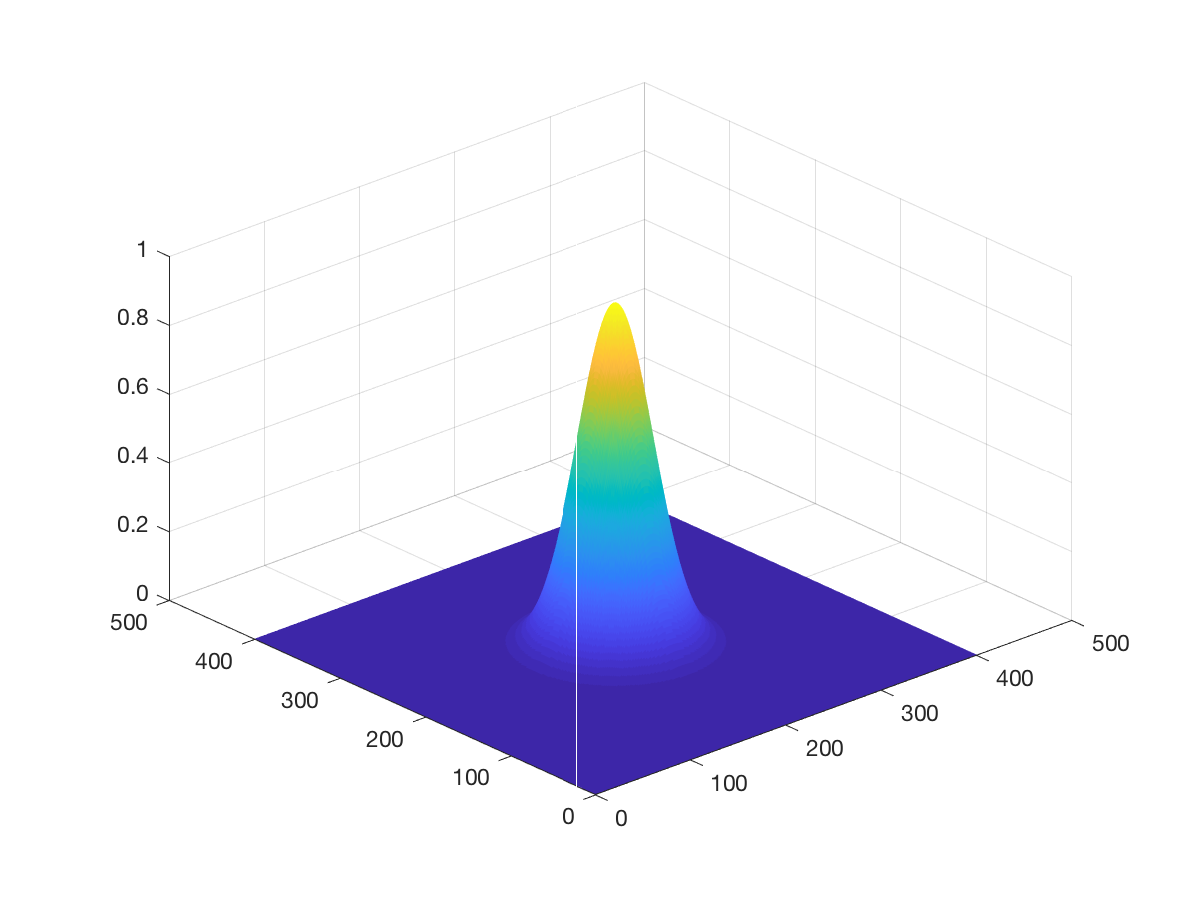
\includegraphics[width=1\linewidth]{figures/part2/gaussian_dis.eps}
		\caption{2D Gaussian}
		\label{fig:gaussian_dis}
	\end{subfigure}
	\begin{subfigure}[t]{0.45\linewidth}
		\centering
		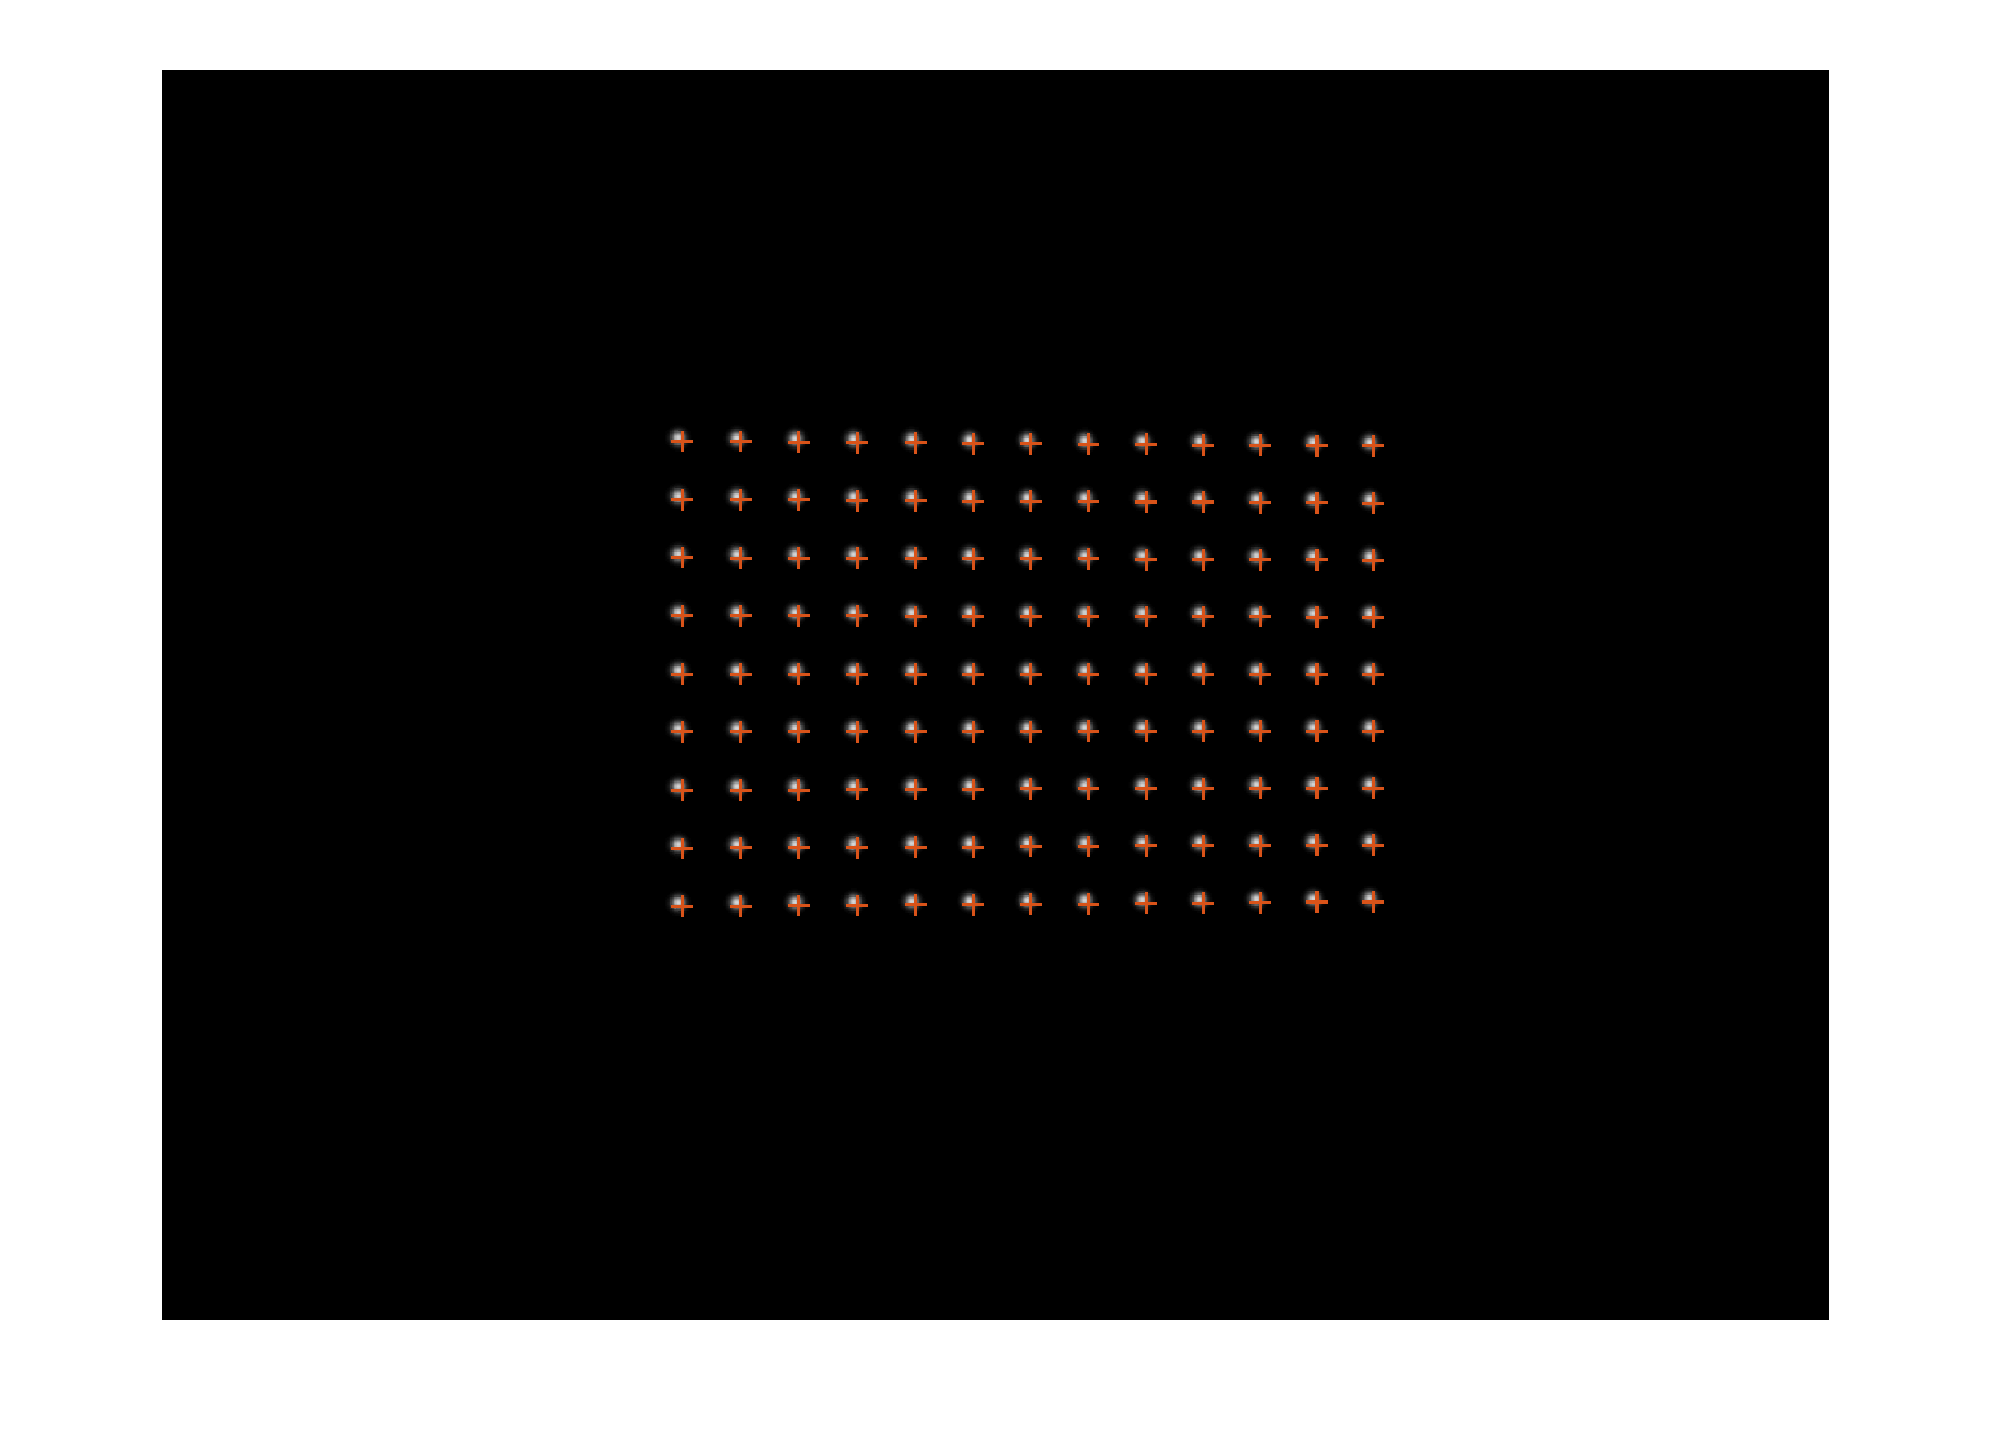
\includegraphics[width=1\linewidth]{figures/part2/dot_detect.eps}
		\caption{Detected dots }
		\label{fig:dot_detect}
	\end{subfigure}
	\caption{Dot Dectection.}
\end{figure}

Detect all dots is not the end of this task. For we need to use these dots in the later work. The points are now stored in the order of its been detected, shown in Figure \ref{fig:dot_disorder}, the read line discribe its storage order. We sort it in order for further using shown like Figure \ref{fig:dot_ordered}.

\begin{figure}[h!]
	\centering
	\begin{subfigure}[t]{0.48\linewidth}
		\centering
		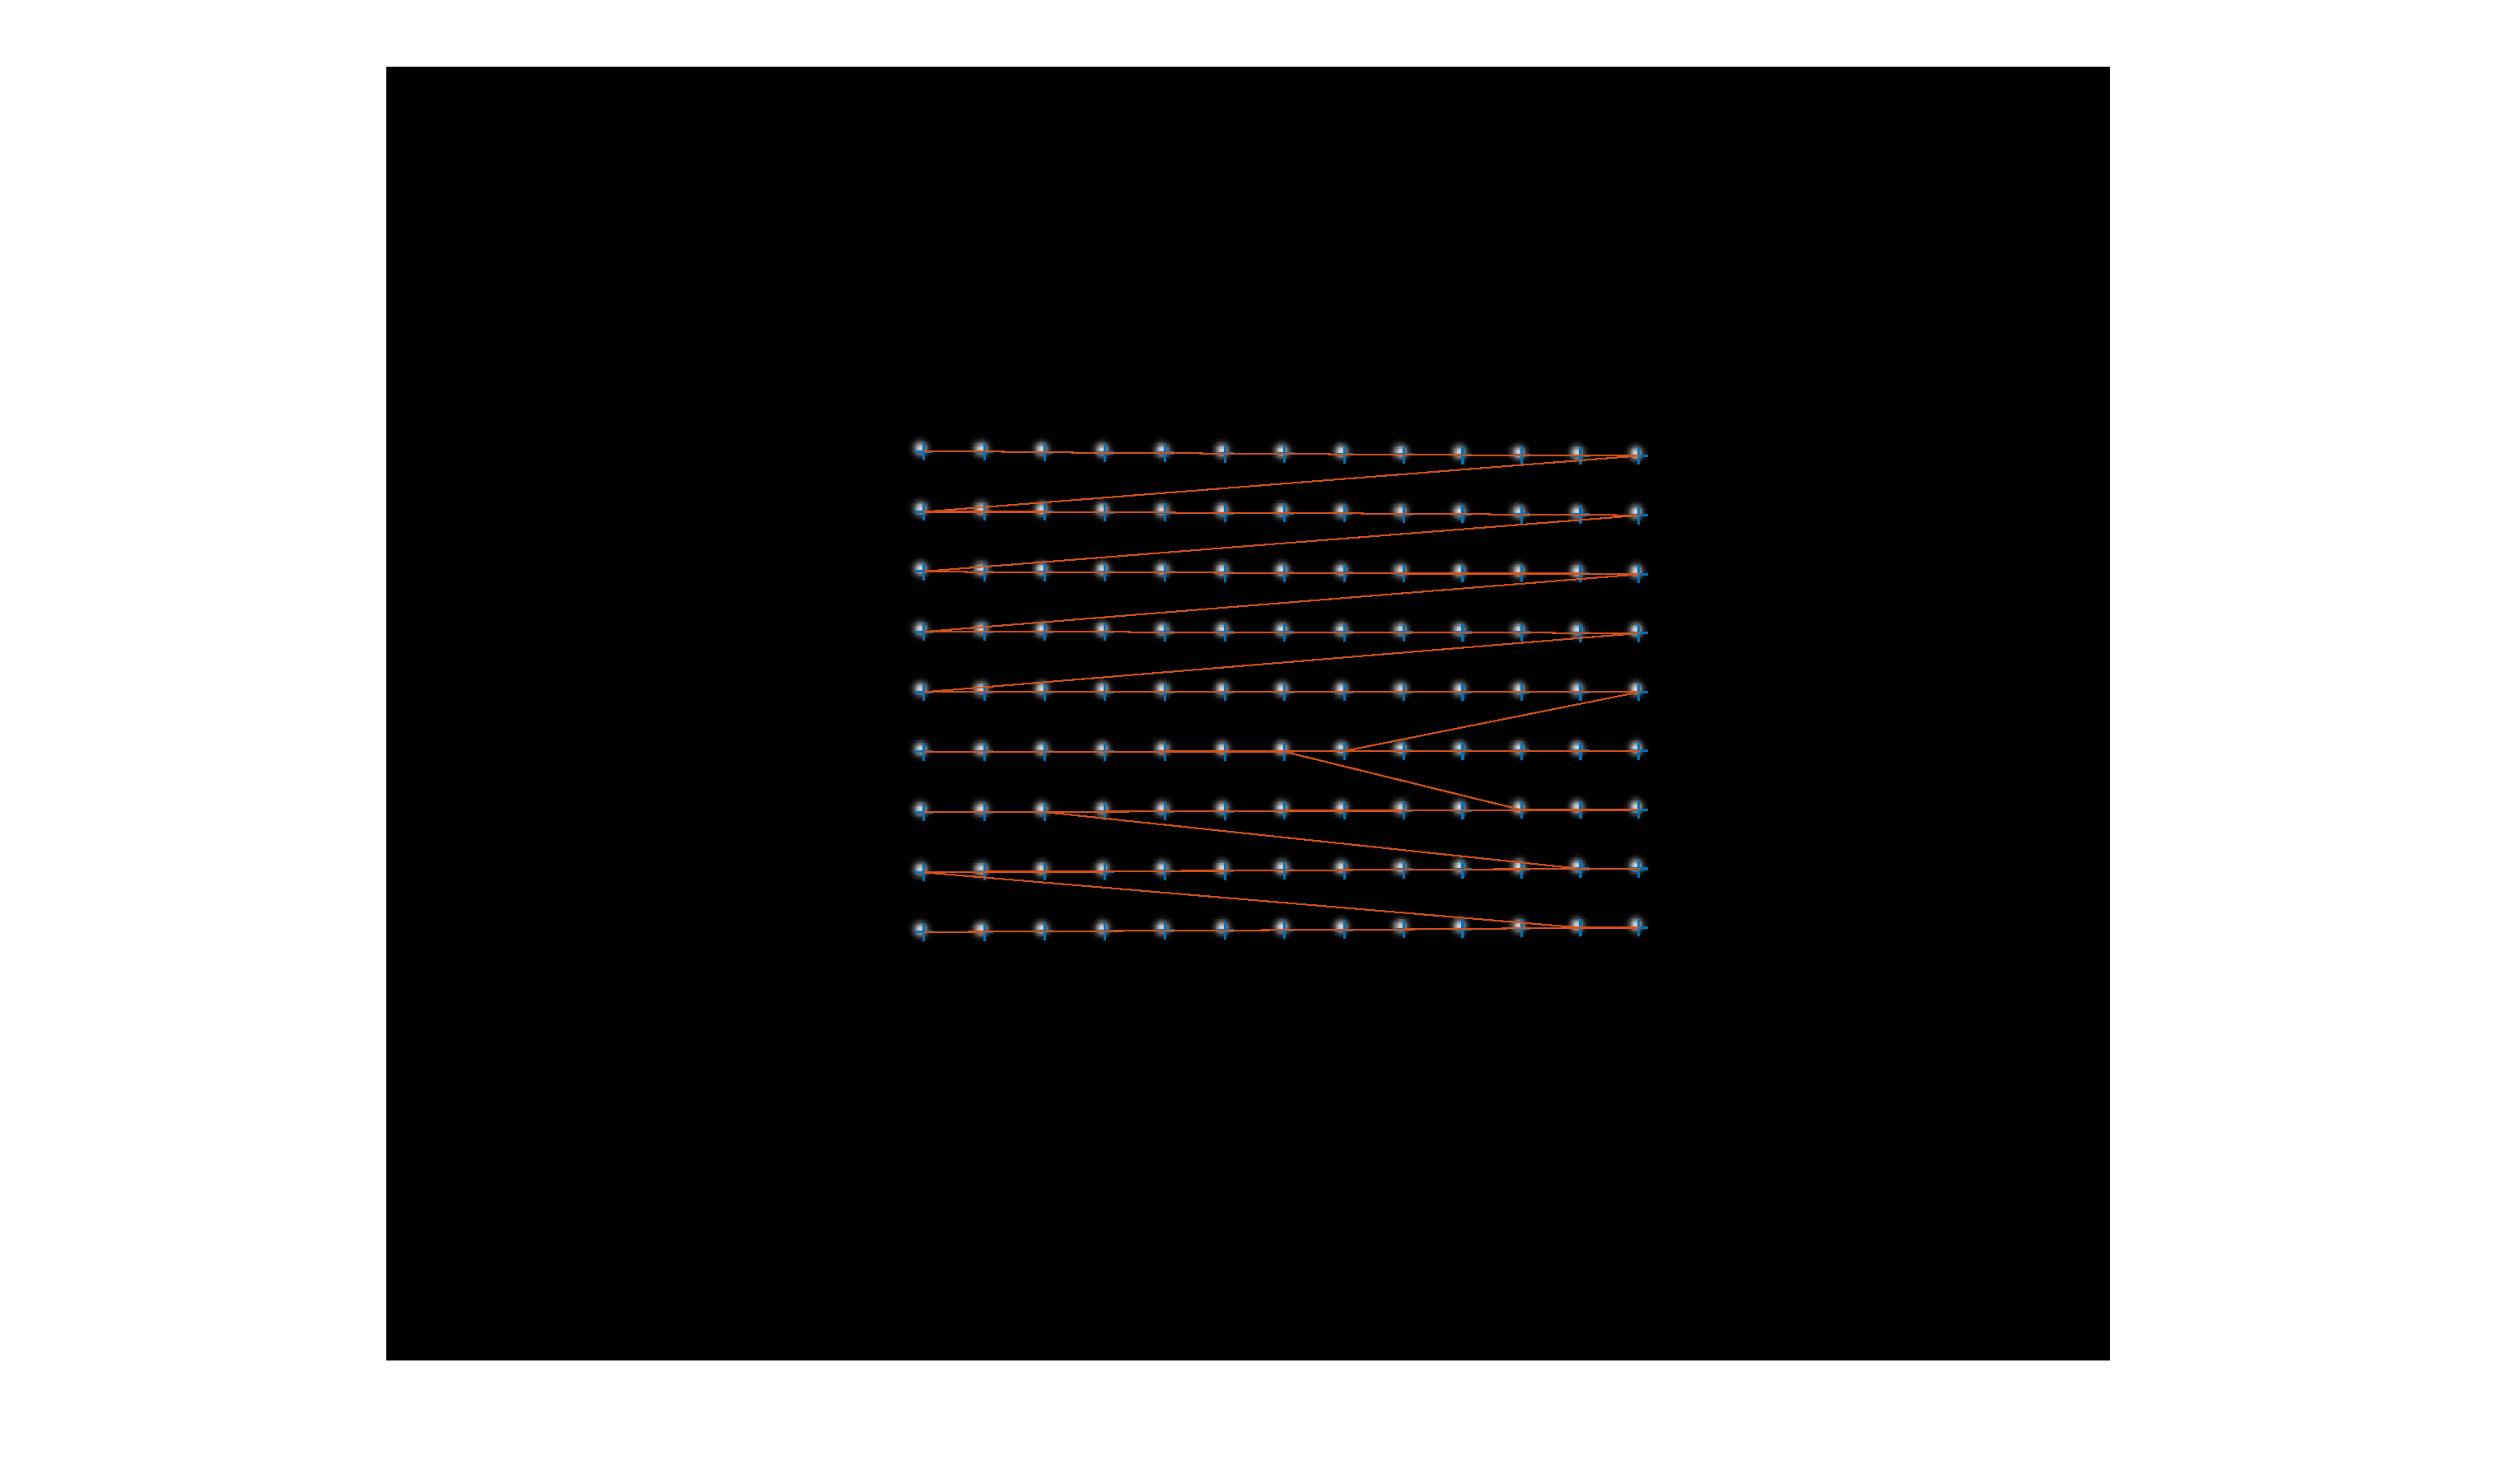
\includegraphics[width=1\linewidth]{figures/part2/dot_disorder.eps}
		\caption{Disordered dots}
		\label{fig:dot_disorder}
	\end{subfigure}
	\begin{subfigure}[t]{0.48\linewidth}
		\centering
		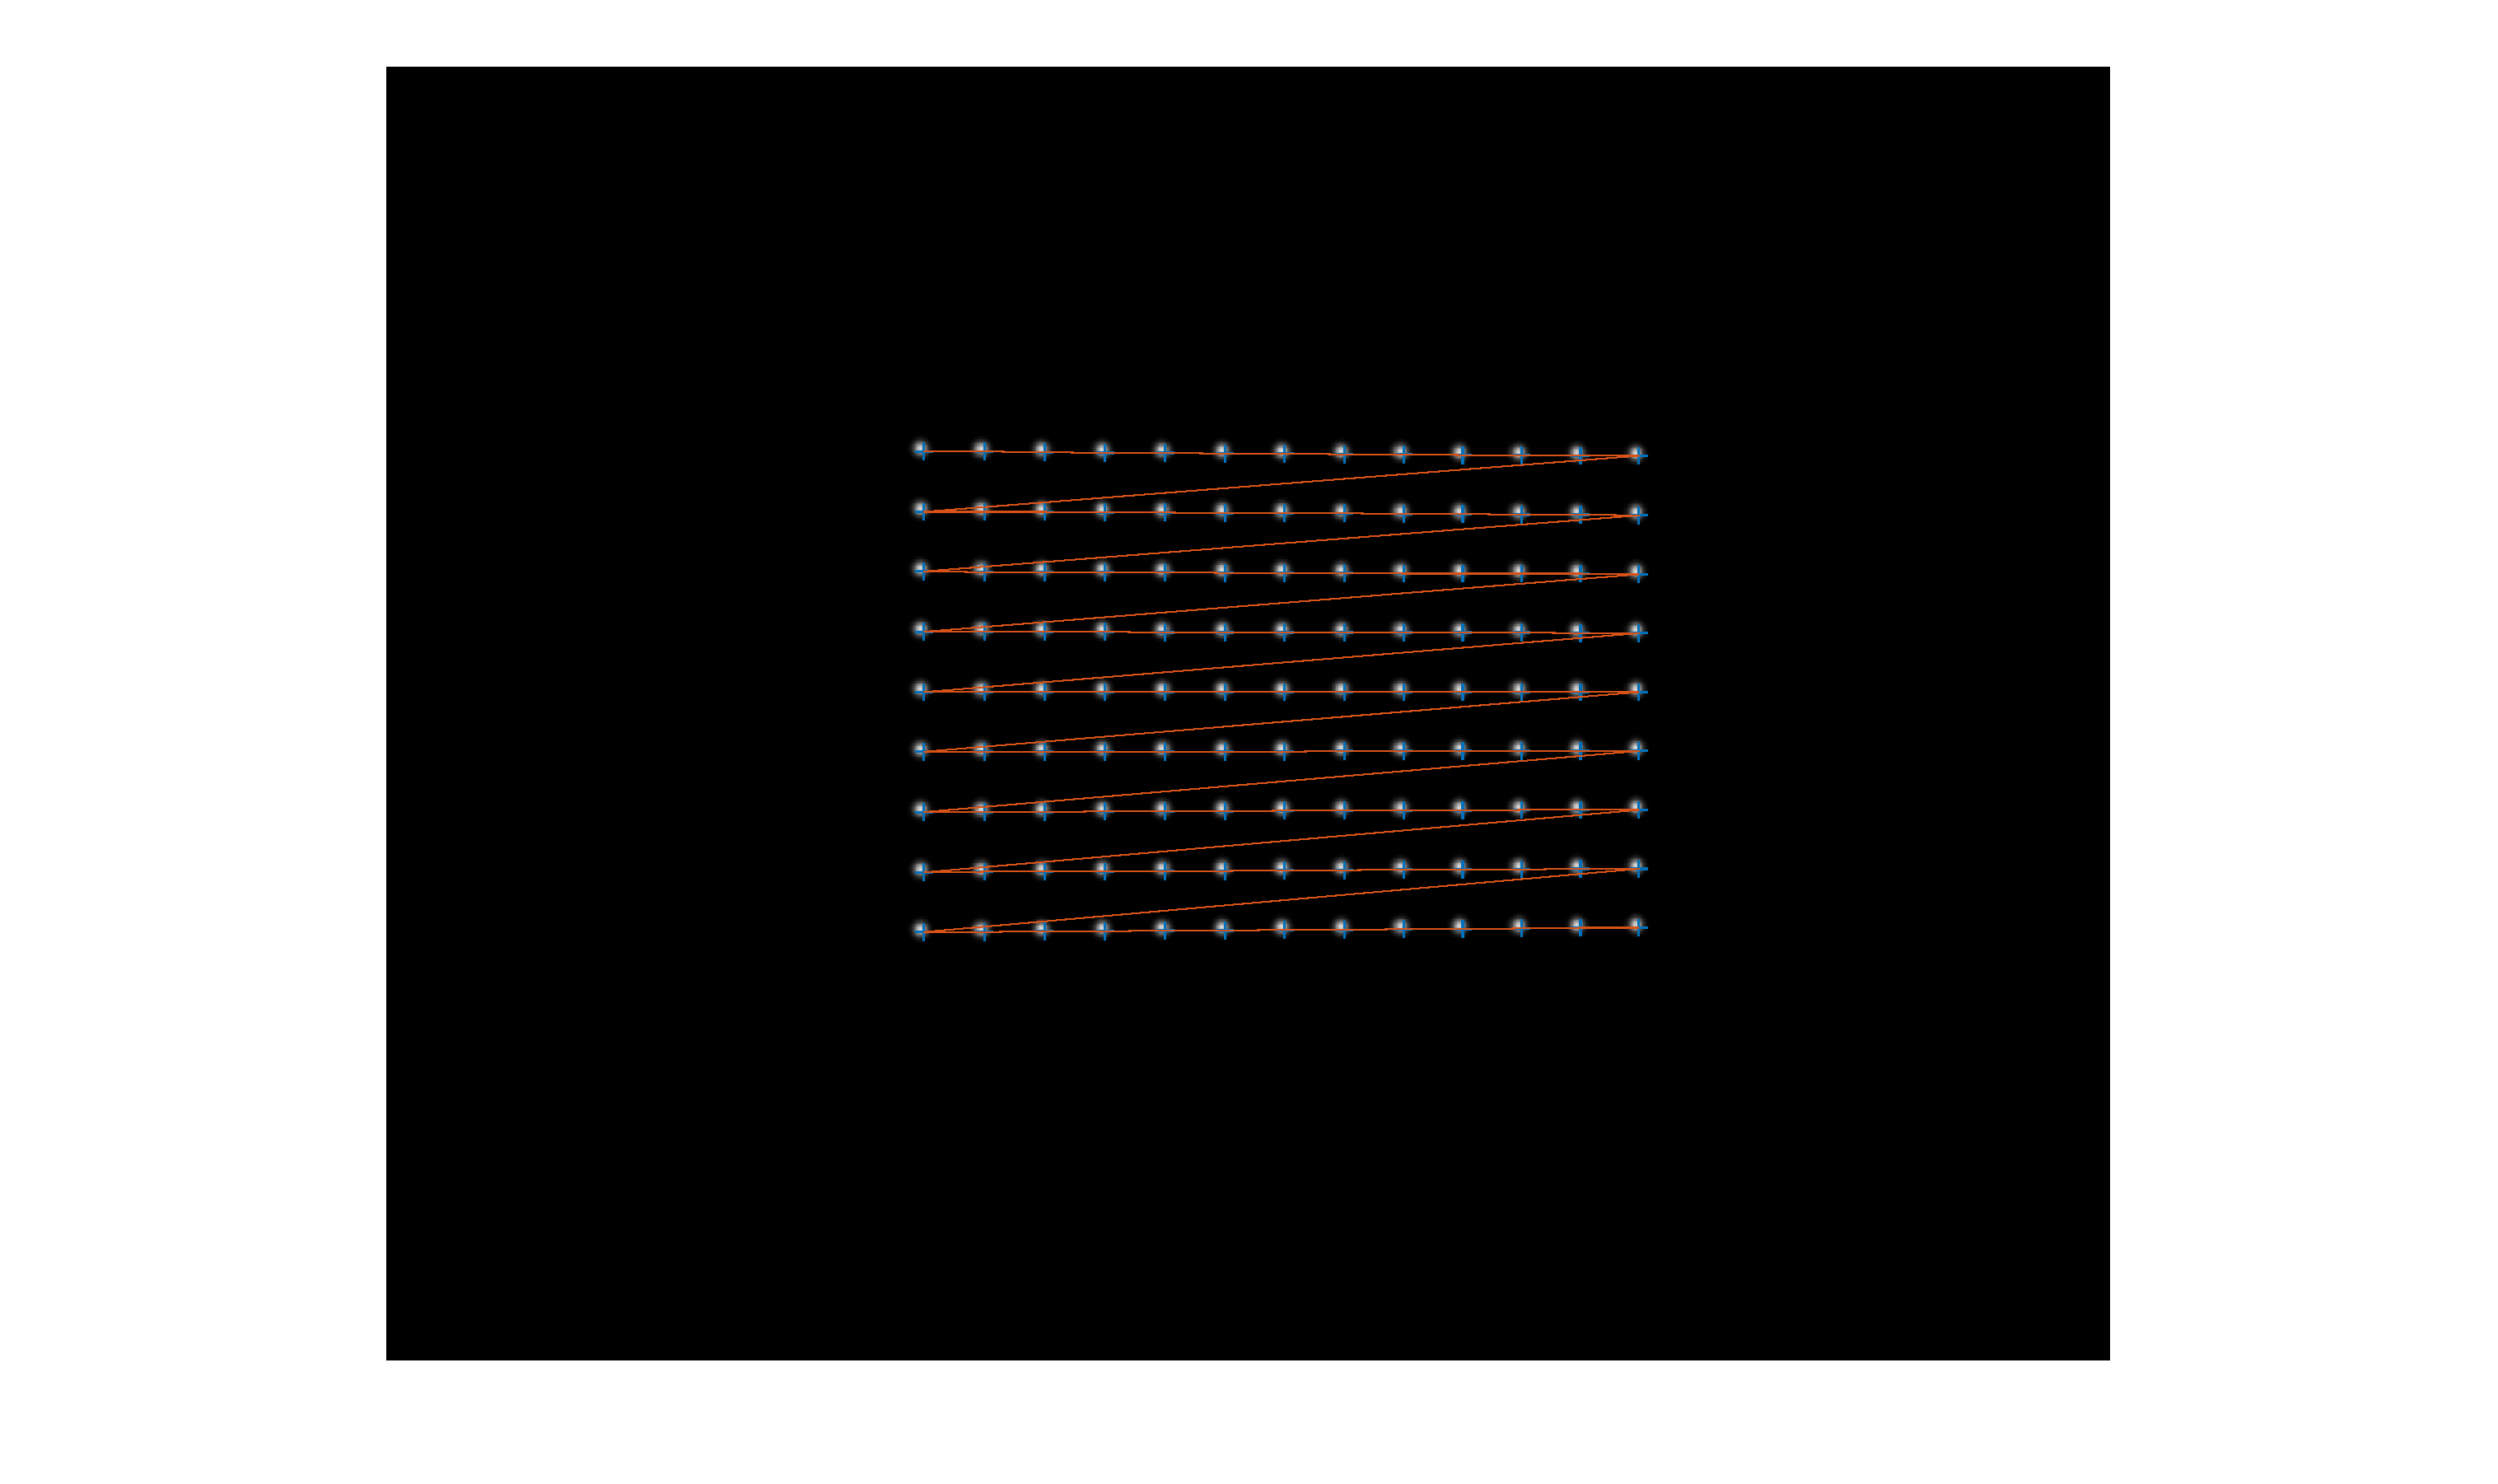
\includegraphics[width=1\linewidth]{figures/part2/dot_ordered.eps}
		\caption{Ordered dots}
		\label{fig:dot_ordered}
	\end{subfigure}
	\caption{Dot Storage.}
\end{figure}

Matlab code of dot detection is in Appendix \ref{code:2.1}.

\section{Create Calibration Model}

Our next step is to create a program which imports all the calibration images and records the pixel and real locations of all of the dots in each image. We use a fitting tool to create a 4D surface fit which connects all pixel space to real space within the calibrated zone. In this task, we have several calibration samples. Each sample contains two images, they are from a left and right camera, viewing the same calibration target at a stereo angle of approximately $\pm9^{\circ}$. The calibration target has white dots spaced by 50 mm in the x (horizontal) and y (vertical) directions. The calibration target is shifted to various z locations and we know the distance of it to the cameras. So the dots' locations in real space is know and their locations in the left and right images can also be detected in task 1. We finally find three funtions to fit $x,y$ and $z$ coordinates in real space by using corresding calibrate target's coordinates in left and right images, as

\begin{equation*}
	\centering
	x_{real} = f_{1}(x_{left}, y_{left}, x_{right}, y_{right}) 
\end{equation*}
\begin{equation*}
	\centering
	y_{real} = f_{2}(x_{left}, y_{left}, x_{right}, y_{right}) 
\end{equation*}
\begin{equation*}
	\centering
	z_{real} = f_{3}(x_{left}, y_{left}, x_{right}, y_{right}) 
\end{equation*}

Matlab code of normalized 1d cross correlation is in Appendix \ref{code:2.2}.

\section{Image Comparision}

After we have build calibration model. We want to apply it to practical scene. But in practice, the images took by camera are not the dots with certain distribution rule. Preprocess of the image is needed before we apply it to our calibration model. Here, we first compare two images take by left and right camera, find corresponding objects in two images.

As we observed in Chapter 1, the cross correlation technique is a very powerful tool which can sensitively and accurately identify patterns in complex images. Consider the two views of Melbourne University as shown in Figure \ref{fig:mel} . As humans, most of us can easily recognise that both images are of the same scene, only taken from different angles or positions. But we must do image comparision to find corresponding objects in two images and then apply it to calibration model.

We first break up one image in to windows and create a template from one window, like shown in Figure \ref{fig:mel_left} , then create a search region (larger than than the template) in the other image as shown in Figure \ref{fig:mel_right}. Then we scan the template around the search region to find similar features using cross correlation,
get the position of max correlation and compute the difference in pixel location. Repeat this for all windows and then we can get all corresponding positions which is very similar with the corresponding dots in task 1 and 2.

\begin{figure}[h!]
	\centering
	\begin{subfigure}[t]{0.48\linewidth}
		\centering
		\includegraphics[width=1\linewidth]{figures/part2/mel_left}
		\caption{Left view}
		\label{fig:mel_left}
	\end{subfigure}
	\begin{subfigure}[t]{0.48\linewidth}
		\centering
		\includegraphics[width=1\linewidth]{figures/part2/mel_right}
		\caption{Right view}
		\label{fig:mel_right}
	\end{subfigure}
	\caption{Template created in left image (orange), search region created in right image (3 times larger than template, centered at the same pixel location).}
	\label{fig:mel}
\end{figure}

Matlab code of normalized 1d cross correlation is in Appendix \ref{code:2.3}.

\section{Cross Correlation Optimisation}

There are several parameters, which need to be considered when applying the cross correlation technique. These include what is the ideal sized window to be used, and how best should it be scanned in search of matching. In this part of the project, we will investigate three optimization strategies:

\begin{itemize}
	\item Window overlap
	\item Search region
	\item Multiple pass
\end{itemize}

\textbf{a). Variable window overlap}
\begin{figure}[h!]
	\centering
	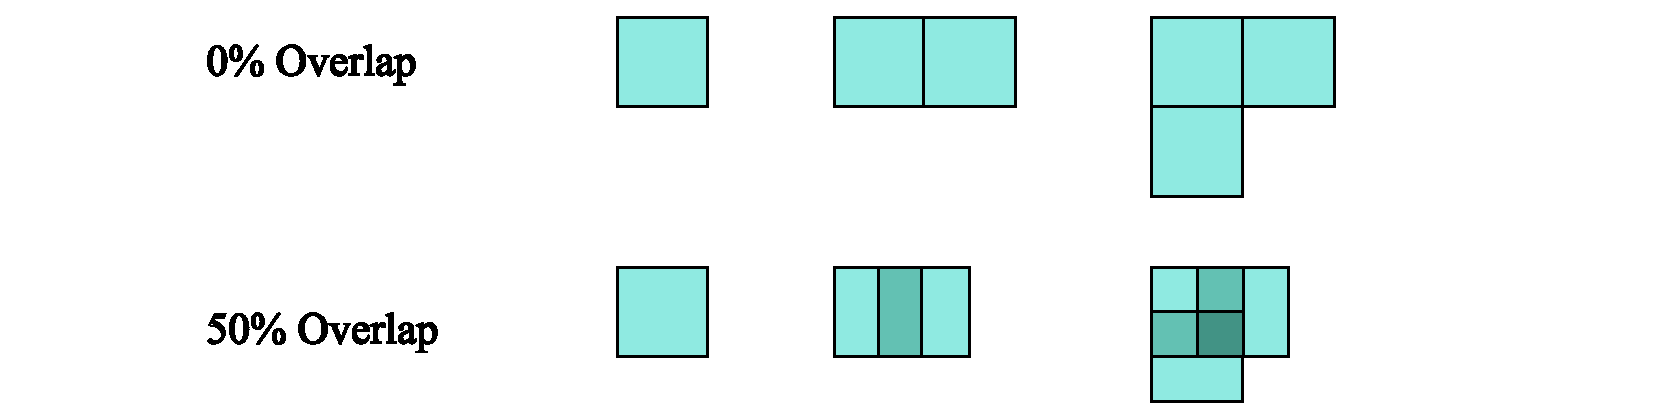
\includegraphics[width=1\linewidth]{figures/part2/window_overlap}
	\caption{Example of variable window operlap}
	\label{fig:window_overlap}
\end{figure}

\textbf{b).Variable search region geometry}
\begin{figure}[h!]
	\centering
	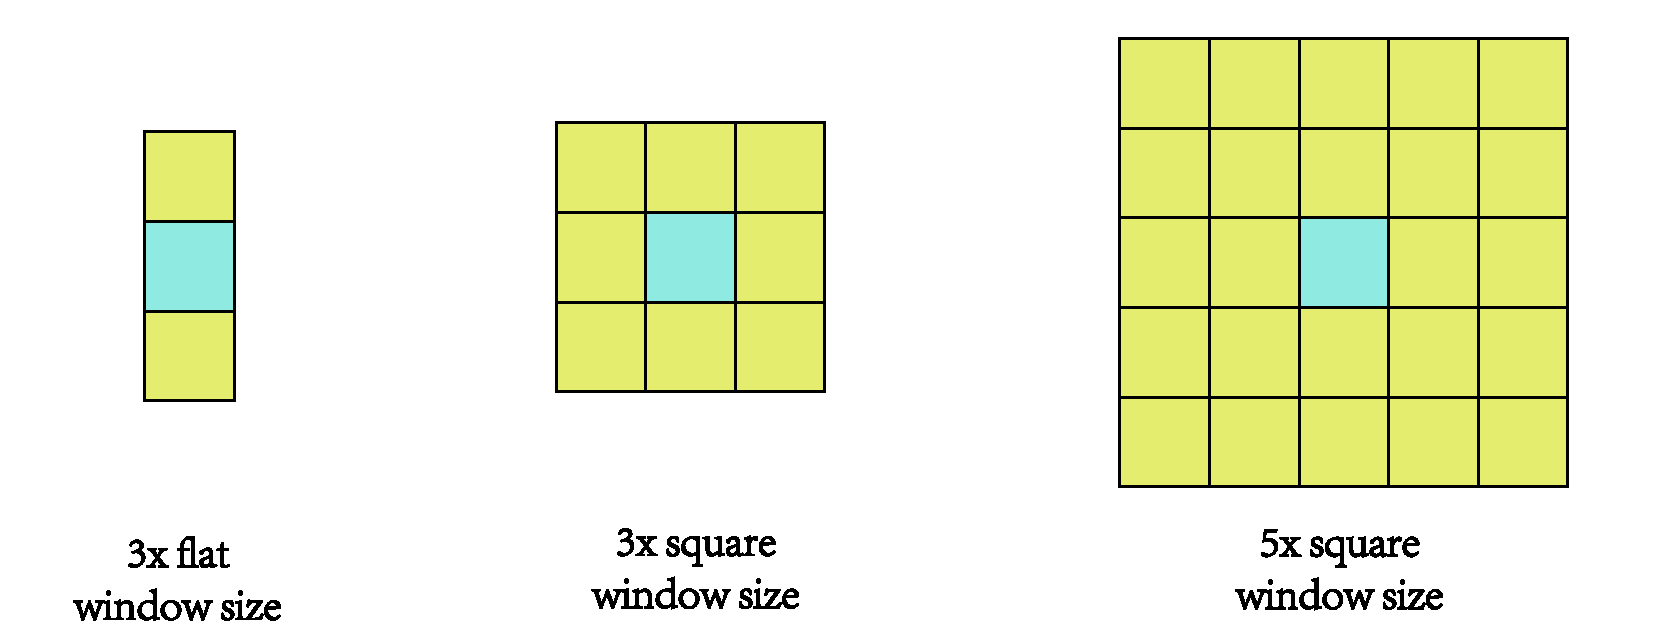
\includegraphics[width=1\linewidth]{figures/part2/search_region}
	\caption{Example of variable search region}
	\label{fig:search_region}
\end{figure}

\textbf{c). Multi-Pass Cross Correlation}
\begin{figure}[h!]
	\centering
	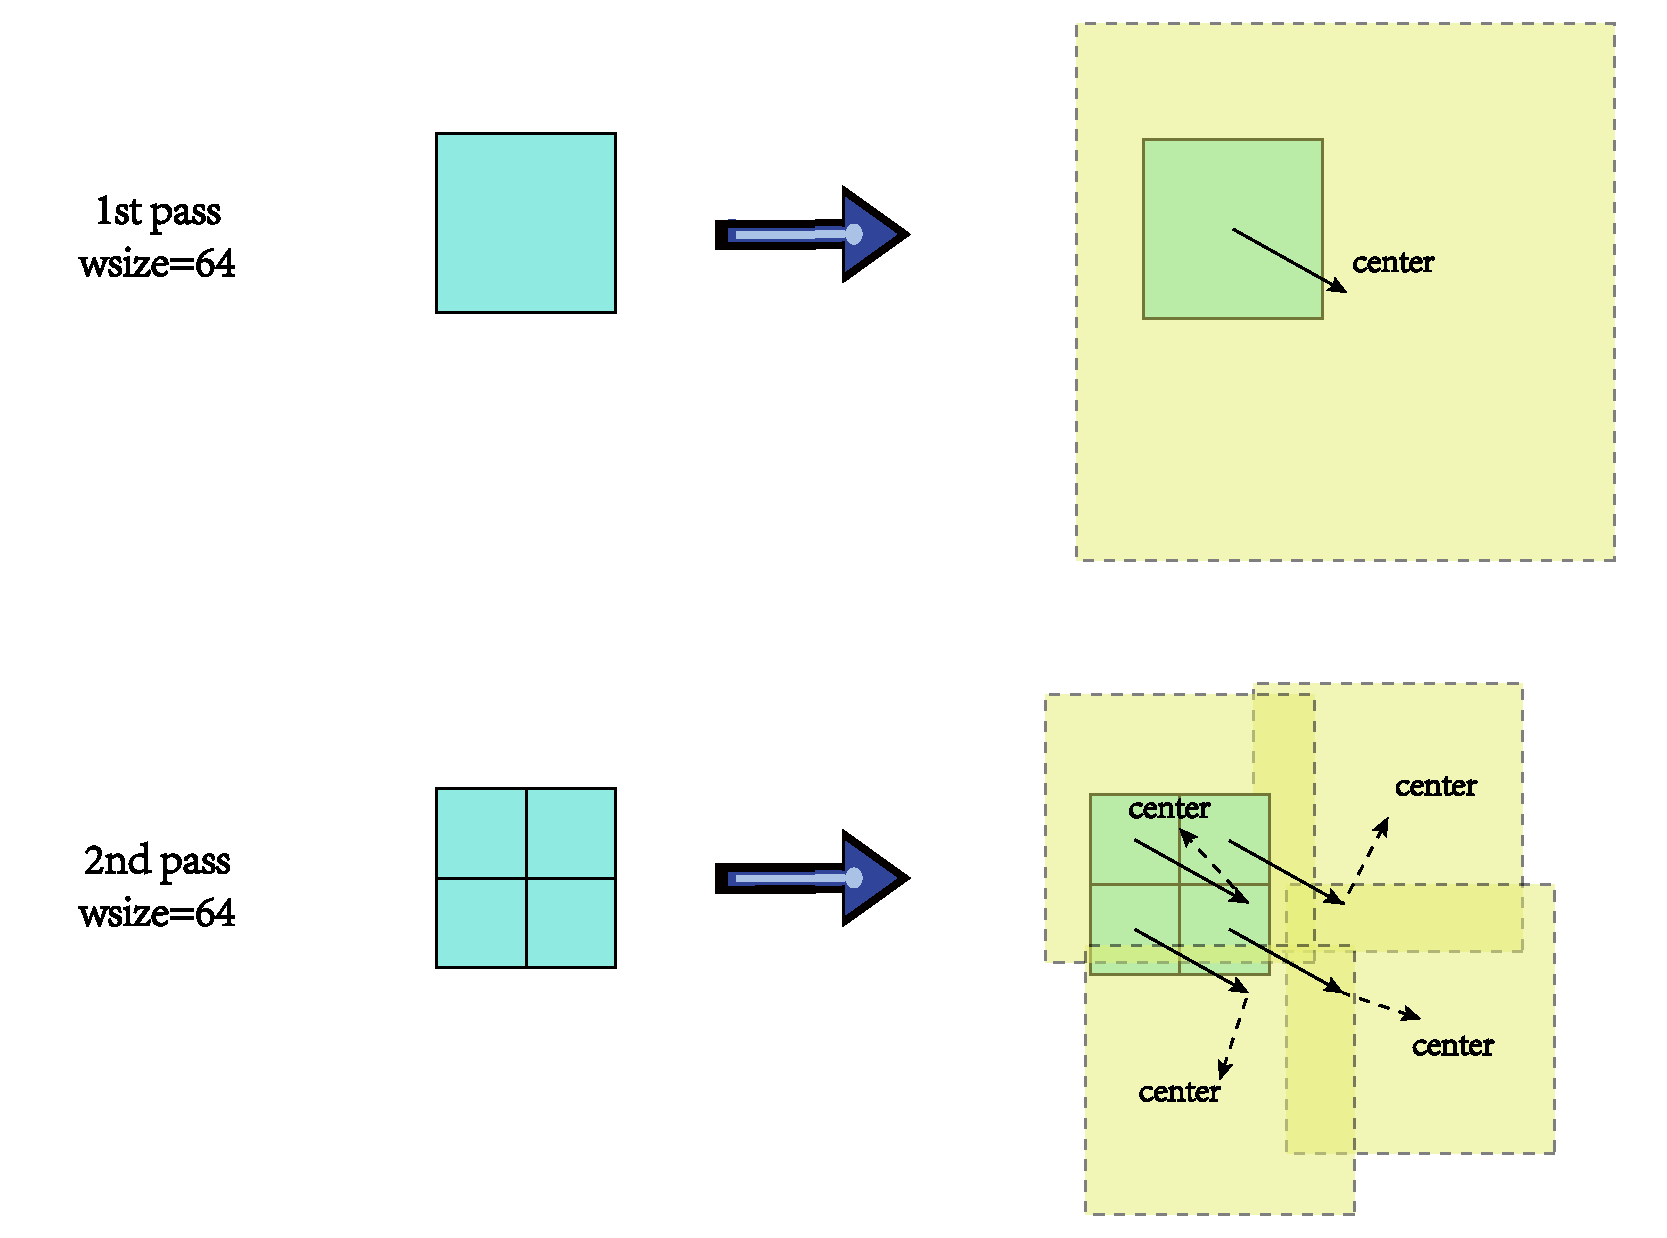
\includegraphics[width=1\linewidth]{figures/part2/multi_pass}
	\caption{Multi pass cross correlation. (``center'' in the image refer to the new search region's center, yellow square is the new search region.)}
	\label{fig:multi_pass}
\end{figure}

Matlab code of normalized 1d cross correlation is in Appendix \ref{code:2.4}.

\section{Test Scan on Computer Generated Calibrated Images}

\section{Optimised Test Scan}